\documentclass[aspectratio=169,11pt]{beamer}

\usepackage[T1]{fontenc}
\usepackage[utf8]{inputenc}
\usepackage[ngerman]{babel}
\usepackage{lmodern}
\usepackage{helvet}
\renewcommand{\familydefault}{\sfdefault}
\usepackage{graphicx}
\usepackage{booktabs}
\usepackage{tikz}
\usetikzlibrary{arrows.meta,positioning}

\usetheme{default}
\usecolortheme{default}
\setbeamertemplate{navigation symbols}{}
\setbeamerfont{frametitle}{size=\Large,series=\bfseries}
\setbeamercolor{frametitle}{fg=black}

\definecolor{aqua}{RGB}{0,90,150}
\setbeamercolor{title}{fg=aqua}
\setbeamercolor{structure}{fg=aqua}

\title{AquaSonic WP5 \\ State Machine Rocket}
\subtitle{Aktueller Stand}
\author{Ahmad Abed Alhady \and Tasnim}
\date{\today}

\begin{document}

% =============================================================================
\begin{frame}
    \titlepage
\end{frame}

% =============================================================================
\begin{frame}{Was gebaut wurde}

    \textbf{Vollst\"andige Sensor-zu-FSM Pipeline in VHDL}

    \vspace{0.6em}
    \begin{center}
    \begin{tikzpicture}[
        node distance=4mm,
        every node/.style={font=\small},
        block/.style={draw=aqua, fill=aqua!10, rounded corners=2pt,
                      minimum width=2.4cm, minimum height=0.7cm, align=center},
        arr/.style={-{Stealth[length=2mm]}, thick, aqua}
    ]
        \node[block] (uart) {uart\_rx \\ \tiny 115200 8N1};
        \node[block, right=of uart] (align) {frame\_aligner \\ \tiny 66 byte};
        \node[block, right=of align] (trig) {trigger\_logic \\ \tiny Debounce};
        \node[block, right=of trig] (fsm) {aquasonic\_fsm \\ \tiny 12 states};

        \draw[arr] (uart) -- (align);
        \draw[arr] (align) -- (trig);
        \draw[arr] (trig) -- (fsm);

        \node[above=1mm of uart, font=\tiny\itshape] {UART line};
        \node[below=1mm of fsm, font=\tiny\itshape] {state\_code + Aktoren};
    \end{tikzpicture}
    \end{center}

    \vspace{0.3em}
    \begin{columns}[T,onlytextwidth]
        \footnotesize
        \column{0.52\textwidth}
        \textbf{Module (6 RTL + 3 TB)}
        \begin{itemize}\setlength{\itemsep}{1pt}
            \item \texttt{aquasonic\_pkg} -- Single Source of Truth
            \item \texttt{uart\_rx} -- 8N1, Mid-Bit-Sampling
            \item \texttt{frame\_aligner} -- Idle-Sync, Field-Extract
            \item \texttt{trigger\_logic} -- 5 Trigger mit Debounce
            \item \texttt{aquasonic\_fsm} -- 3-Prozess, latch-frei
            \item \texttt{rocket\_top} -- Verdrahtung
        \end{itemize}

        \column{0.45\textwidth}
        \textbf{Highlights}
        \begin{itemize}\setlength{\itemsep}{1pt}
            \item Keine Floats / kein sqrt im RTL
            \item Alle Schwellwerte in einer Datei
            \item Spec-konforme 4-bit State-Codes
            \item Self-checking Testbenches
        \end{itemize}
    \end{columns}

\end{frame}

% =============================================================================
\begin{frame}{Tests \-- alle drei Simulationen sauber}

    \begin{center}
    \small
    \begin{tabular}{@{}lll@{}}
        \toprule
        \textbf{Test}                  & \textbf{Was wird gepr\"uft}            & \textbf{Status} \\
        \midrule
        \texttt{sim\_fsm.do}           & 12 States, 4 Test-Gruppen              & \textcolor{aqua}{\textbf{OK}} \\
        \texttt{sim\_trigger.do}       & 5 Trigger + Debounce                   & \textcolor{aqua}{\textbf{OK}} \\
        \texttt{sim\_top.do}           & End-to-End mit echter Flugdaten-CSV    & \textcolor{aqua}{\textbf{OK}} \\
        \bottomrule
    \end{tabular}
    \end{center}

    \vspace{0.6em}

    \begin{columns}[T,onlytextwidth]
        \column{0.48\textwidth}
        \centering
        \textbf{FSM Transcript}\\[2pt]
        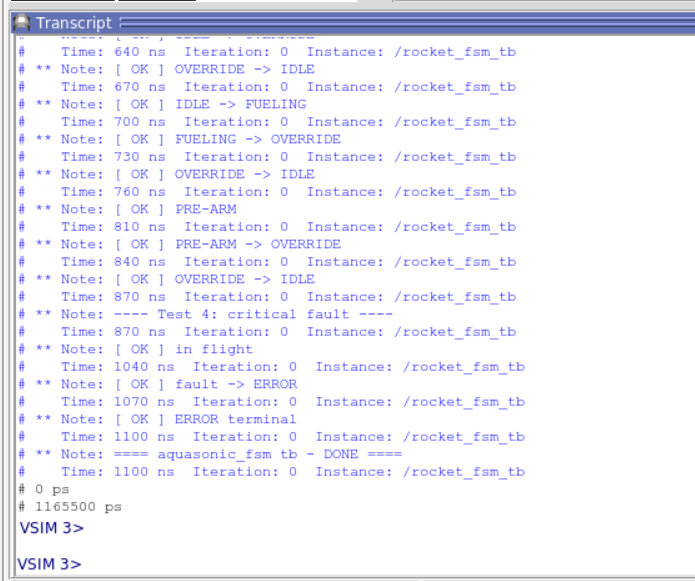
\includegraphics[width=\linewidth,height=4.4cm,keepaspectratio]{screenshots/fsm_transcript.png}

        \column{0.48\textwidth}
        \centering
        \textbf{Integration mit CSV}\\[2pt]
        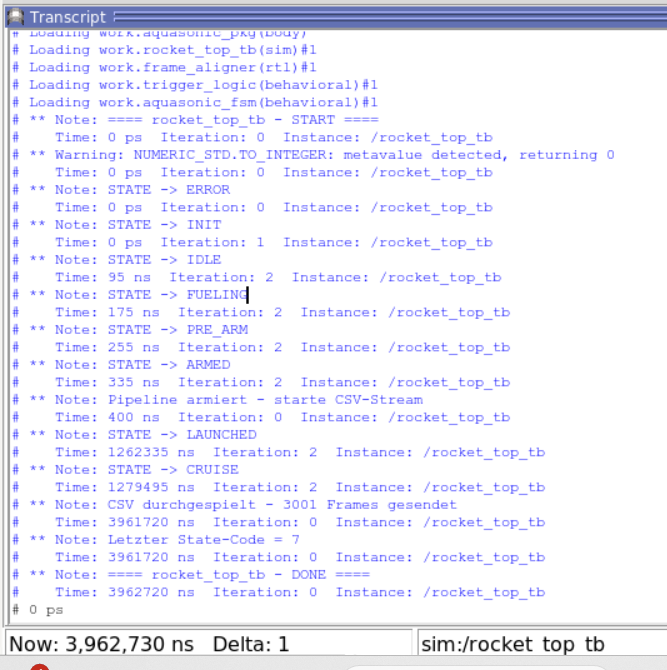
\includegraphics[width=\linewidth,height=4.4cm,keepaspectratio]{screenshots/top_transcript.png}
    \end{columns}

    \vspace{0.4em}
    \footnotesize Detailprotokoll: \texttt{docs/TEST\_LOG.md}

\end{frame}

% =============================================================================
\begin{frame}{Was die echte CSV liefert \-- und was fehlt}

    \begin{columns}[T,onlytextwidth]
        \column{0.55\textwidth}
        \centering
        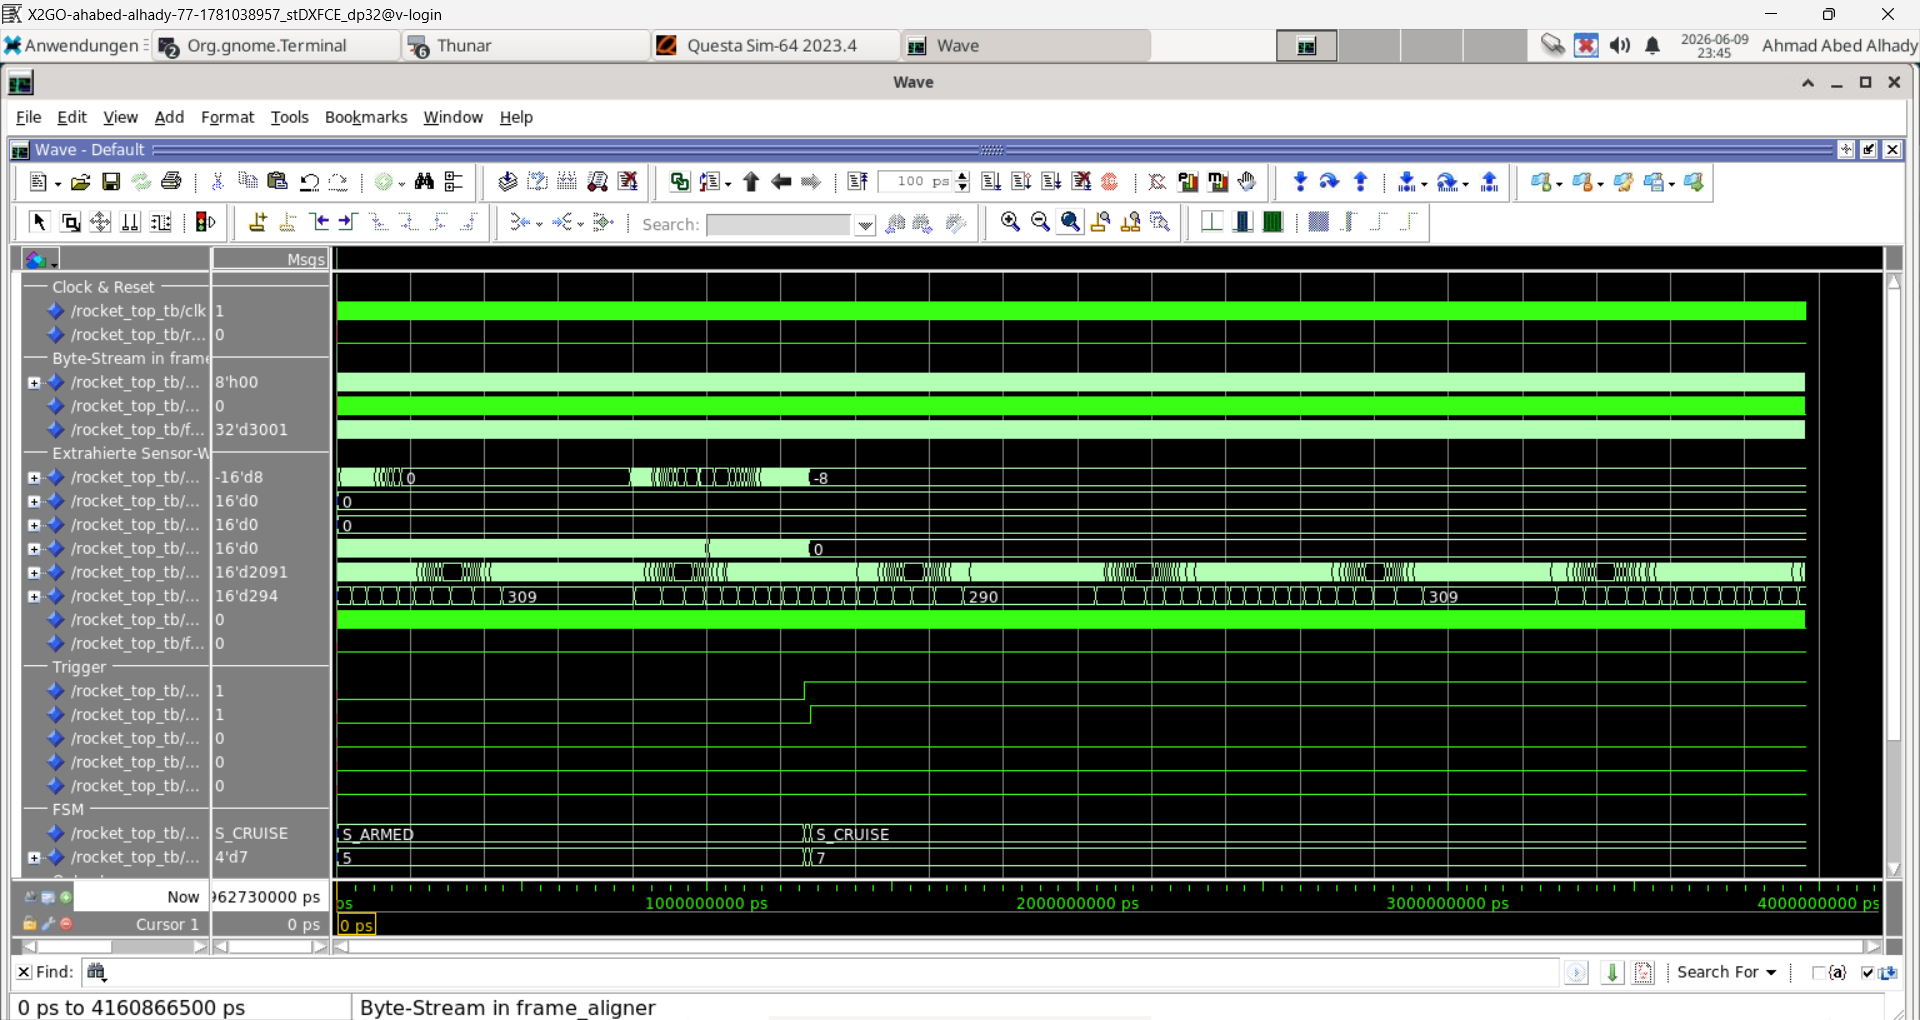
\includegraphics[width=\linewidth,height=5.0cm,keepaspectratio]{screenshots/top_wave.png}\\
        \footnotesize \texttt{sim\_top.do} Wave-Ansicht

        \column{0.42\textwidth}
        \textbf{Ergebnis aus 3001 Frames}
        \begin{itemize}\setlength{\itemsep}{2pt}
            \item Pipeline l\"auft bis \textbf{CRUISE} (Code 7)
            \item Liftoff feuert bei Zeile 954
            \item Burnout feuert bei Zeile 967
            \item Apogee / Main / Landed nicht
        \end{itemize}

        \vspace{0.4em}
        \textbf{Warum?}\\
        CSV endet ab Zeile $\sim$964 mit \texttt{baro\_h = 0} \-- Sensor-Ausfall im Originaldatensatz. \textbf{Kein RTL-Bug.}

        \vspace{0.4em}
        \textbf{Was wir brauchen}\\
        Kompletter Flugdatensatz mit Apogee, Recovery und Touchdown vom Rocket-Team.
    \end{columns}

\end{frame}

% =============================================================================
\begin{frame}{Stand \& n\"achste Schritte}

    \begin{columns}[T,onlytextwidth]
        \column{0.48\textwidth}
        \textbf{Erledigt}
        \begin{itemize}\setlength{\itemsep}{2pt}
            \item Komplette Pipeline implementiert
            \item Drei Testbenches funktionsf\"ahig
            \item Integrationstest mit Echtdaten
            \item Konstanten zentralisiert (Package)
            \item Doku: README, ARCHITECTURE, TEST\_LOG
        \end{itemize}

        \column{0.48\textwidth}
        \textbf{Offen}
        \begin{itemize}\setlength{\itemsep}{2pt}
            \item Kompletter Flugdatensatz f\"ur Apogee--Landed Test
            \item Schwellwerte final vom Rocket-Team (Tank TBD)
            \item Vivado-Synthese auf Trenz Z7020
            \item Operator-Command-Decoder mit AquaCom-Team
            \item \texttt{telemetry\_tx}-Modul (state\_code zur\"uck in Paket)
        \end{itemize}
    \end{columns}

    \vspace{0.9em}
    \begin{center}
    \begin{tikzpicture}
        \node[draw=aqua, fill=aqua!10, rounded corners=3pt, inner sep=8pt, align=center]
            {\textbf{Status:} VHDL-Implementierung funktional verifiziert und abgabe-bereit.\\
             Bereit f\"ur Synthese sobald Schwellwerte final sind.};
    \end{tikzpicture}
    \end{center}

\end{frame}

\end{document}
